\documentclass{beamer}
\usepackage{amsmath, amsfonts, amssymb, amsthm}
\usepackage{graphicx, caption, hyperref, url, cite}
\usepackage[UTF8, noindent]{ctexcap}
\usepackage{listings}

\usetheme{Boadilla}

\title{汇报0525}
% \subtitle{项目三:基于大规模预训练模型的生成式知识问答}
\institute{项目三}
\author{朱睿涵 \and 李宸亦}
\date{\today}

\setbeamertemplate{bibliography item}[text]

\begin{document}

\frame{\titlepage} % 标题页

\AtBeginSection{
    \begin{frame}
        \frametitle{目录}

        \tableofcontents[currentsection]
    \end{frame}
}


\section{调研CoQA数据集}
\begin{frame}
    \frametitle{CoQA简介}
    CoQA A Conversational Question Answering Challenge

    CoQA:一个用于建立对话式问题回答(Conversational Question Answering)系统的新型数据集。
    数据集包含12.7万个带答案的问题,这些问题来自7个不同领域的8千条文本段落的对话,后续实验中五个用于域内评估,两个用于域外评估。
    问题是对话式的,而答案是自由格式的文本,并在段落中突出了相应的证据。

\end{frame}


\begin{frame}
    \frametitle{CoQA开发目标}
    \begin{itemize}
        \item 还原人类对话的性质:人们在日常对话中很少像阅读理解一样,基于材料生搬硬套出一个答案,
                要还原对话的这一本质,就需要解决传统阅读理解问题的问题-文章依赖性,以及实现基于对话历史的问答
        \item 确保对话中答案的自然度:以往的阅读理解会依赖材料截取答案,导致答案不够自然,不够口语化。因此要通过CoQA训练出形式较为自由的抽象答案,而不是简单的信息提取。
        \item 建立跨领域表现稳健的QA系统:以往的QA数据集来源于单一领域而CoQA的数据来源于七个领域
    \end{itemize}

\end{frame}

\begin{frame}
    \frametitle{目标任务}
    给定一篇文章和一段对话,回答对话中的下一个问题。
    对话中的每一轮由问题(Q),答案(A),依据(R)组成,答案往往比依据简洁很多。

    回答问题时,需要考虑对话中的历史信息,比如回答$Q_2$时,要基于对话历史$Q_1,A_1$以及答案依据$R_2$,可表示为:

    $$ A_2 = f(Q_1,A_1,Q_2,R_2) $$

    $$ A_n = f(Q_1,A_1,...,Q_{n-1},A_{n-1},R_n,Q_n) $$

    对于无法回答的问题,给出“unknown”的回答,不标注任何依据(R)

\end{frame}

\begin{frame}
    \frametitle{数据收集}
    提出新的问题者,希望避免使用段落中的确切词汇,以增加词汇的多样性。
    当他们输入一个已经出现在段落中的词时,提醒他们尽可能地转述问题。界面如图:
    \begin{figure}[tb]
        \centering
        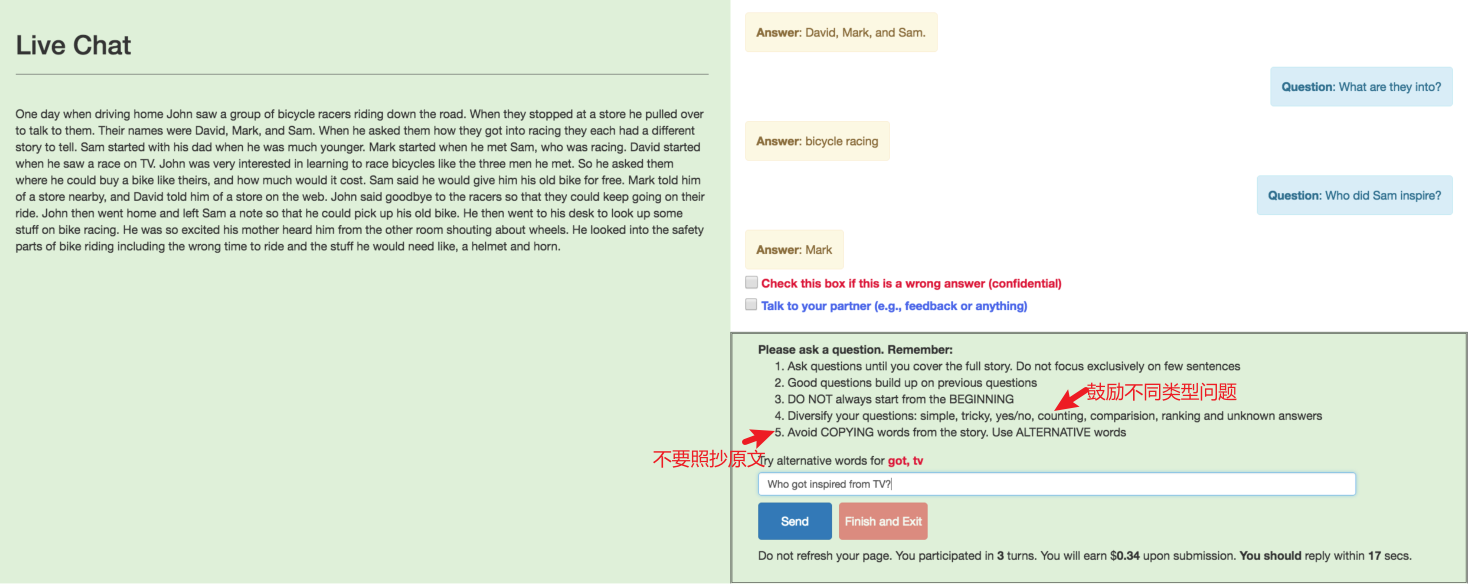
\includegraphics[width=0.9\textwidth]{fig/interface1.png}
    \end{figure}
\end{frame}

\begin{frame}
    \frametitle{数据收集}
    回答问题者,希望回答者坚持使用段落中的词汇,以限制可能的答案数量。界面如图:
    \begin{figure}[tb]
        \centering
        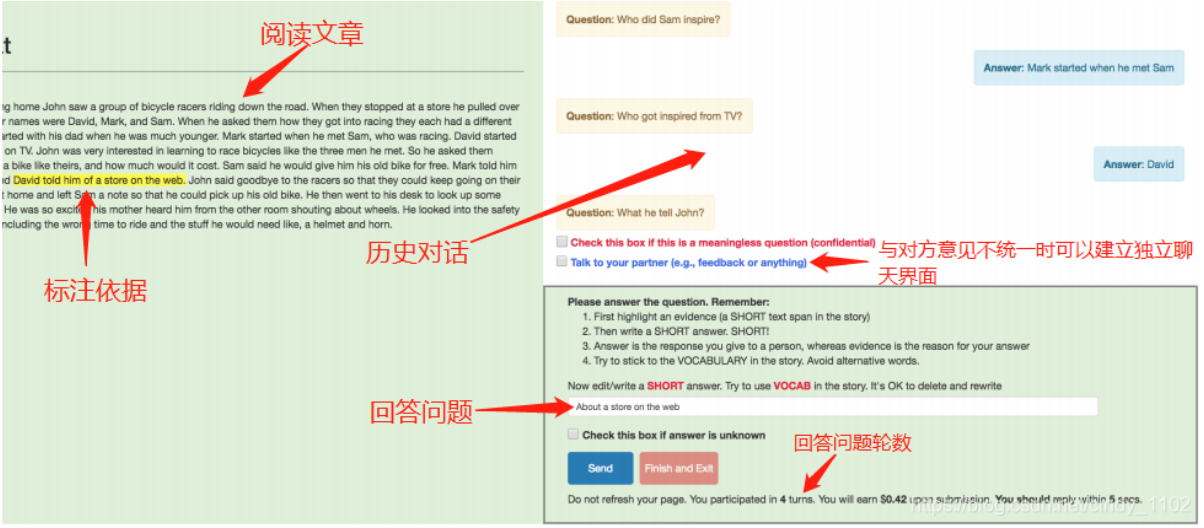
\includegraphics[width=0.9\textwidth]{fig/interface2.png}
    \end{figure}
\end{frame}

\begin{frame}
    \frametitle{数据集划分}
    选取儿童故事、文学、初中和高中英语考试、新闻、维基百科、Reddit和科学7个方面。
    \begin{figure}[tb]
        \centering
        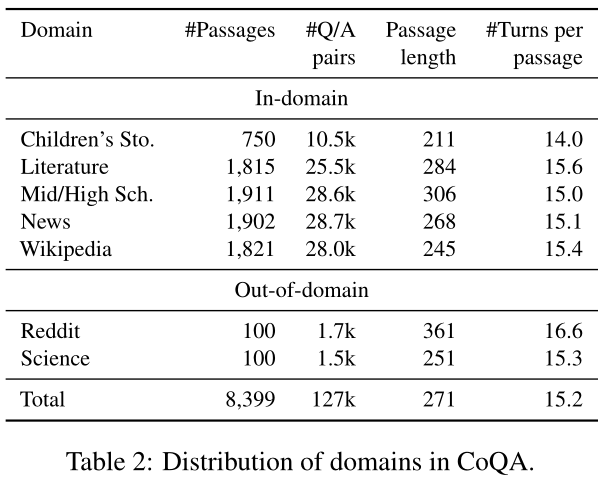
\includegraphics[width=0.5\textwidth]{fig/datafrom.png}
    \end{figure}
    数据集划分:

    对于领域1-5: 开发集100篇文章,测试集100篇文章,其余文章作为训练集

    对于领域6-7: 测试集100篇文章,其余文章作为训练集
\end{frame}

\begin{frame}
    \frametitle{模型}
    \begin{block}{模型}
    给定段落p

    对话历史${q_1,a_1,...,q_{i-1},a_{i-1}}$

    黄金答案$a_1,a_2,...,a_{i-1}$被用来预测$a_i$

    输入:问题$q_i$

    输出:答案$a_i$

    模型:PGNet,DrQA,PGNet+DrQA
    \end{block}

    组合模型中,阅读理解模型DrQA首先指出文本中的答案证据,而对话模型PGNet则将证据归化为答案。
    根据经验对DrQA和PGNet做了一些改变。对于DrQA,如果答案是理由的一个子串则直接预测答案,否则就预测理由。
    对于PGNet,提供当前问题和DrQA的跨度预测作为编码器的输入,解码器的目的是预测最终的答案。

\end{frame}

\begin{frame}
    \frametitle{结果}
    \begin{figure}[tb]
        \centering
        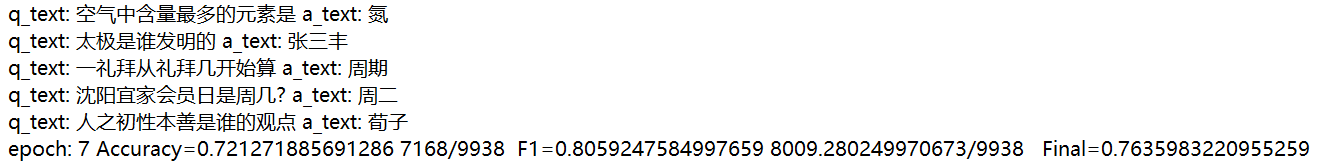
\includegraphics[width=0.7\textwidth]{fig/result.png}
    \end{figure}
    \begin{enumerate}
        \item seq2seq模型的表现最差
        \item 组合模型优于两者的单一模型,可以与增强的DrQA相比较
        \item 最好的模型比人类表现差
    \end{enumerate}
\end{frame}

\begin{frame}
    \frametitle{分析点}
    \begin{figure}[tb]
        \centering
        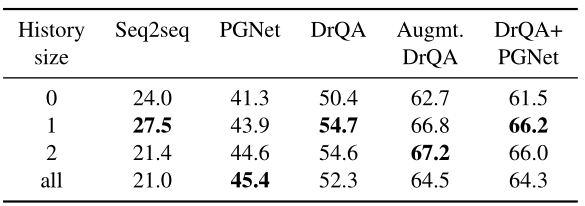
\includegraphics[width=0.7\textwidth]{fig/ana.png}
    \end{figure}
    所有的模型都成功地利用了历史,但超过一个以前的回合,收益就很少了。随着我们增加历史记录的大小,性能会下降。
    在人的实验中,前一回合在理解当前问题中起着重要作用;对话中的大多数问题在两个回合的范围内有有限的依赖性。
\end{frame}


\section{调研百度千言数据集}
\begin{frame}
    \frametitle{百度千言数据集}
    百度千言针对阅读理解任务有三个数据集,其中Dureader checklist和DuReader robust是单篇章、抽取式阅读理解数据集,
    DuReader yesno是观点型的。


\end{frame}

\begin{frame}[fragile]
    \frametitle{百度千言数据集}
    \begin{lstlisting}[]

DuReader yesno的数据集:
{
"documents": [
    {
    "title": "香蕉能放冰箱吗 香蕉剥皮冷冻保存_健康贴士_保健_99健康网",
    "paragraphs": [
        "本文导读:............."
    ]
    }
],
"yesno_answer": "No",
"question": "香蕉能放冰箱吗",
"answer": "香蕉不能放冰箱,香蕉如果放冰箱里,
        会更容易变坏,会发黑腐烂。",
"id": 293
}
    \end{lstlisting}

\end{frame}

\begin{frame}[fragile]
    \frametitle{百度千言数据集}

    checklist和robust的数据集:

    \begin{figure}[tb]
        \centering
        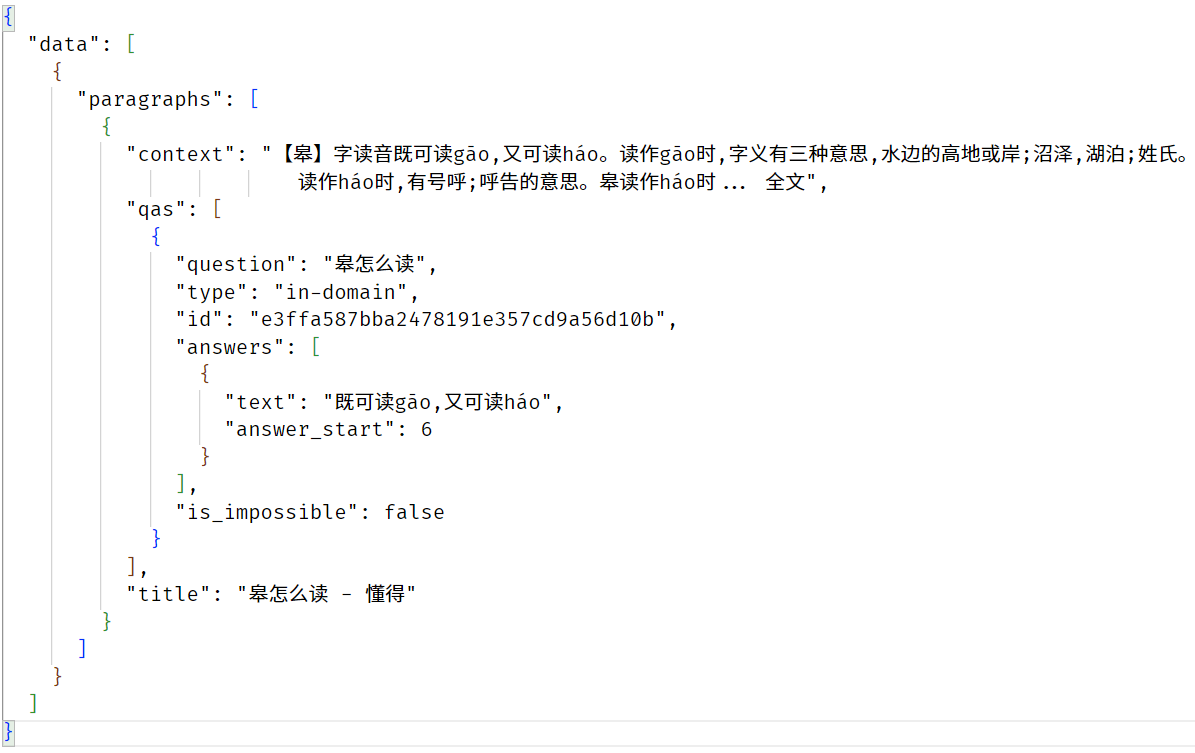
\includegraphics[width=0.9\textwidth]{fig/data.png}
    \end{figure}

\end{frame}

\begin{frame}
    \frametitle{百度千言数据集}

    checklist和robust和之前用过的数据集类型差不多意义不是很大,也许可以作为训练和测试的补充。
    DuReader yesno这种观点型的数据集和之前的类型不同,把DuReader yesno装进模型训练的意义更大一些。

\end{frame}


\section{移植baseline}
\begin{frame}
    \frametitle{baseline}
    上周对于苏剑林baseline进行了简单的pytorch改写,为保证之后基于此baseline的微调工作能够顺利进行,
    本周继续完成对于baseline的改写工作.

    本周对于我们改写过的baseline模型又进行了结构化调整,消除了之前存在的一些潜在问题,
    目前baseline从keras到pytorch的移植工作基本完成,如果下周计算资源申请到位后可以进行模型微调和数据集的加入.

\end{frame}



\begin{frame}
    THANKS!


\end{frame}

% \begin{frame}{References}

%     \nocite{*}
%     \bibliographystyle{unsrt}
%     \bibliography{reference.bib}

% \end{frame}
\end{document}
